\section{Algoritmo Formiga}

 O primeiro sistema formiga para VRP foi desenhado muito recentemente por {\color{red} referência},
o qual considera a versão mais elementar do problema: CVRP.

 Para mais versões mais complexas de VRP, {\color{red} referência} tem desenvolvido um sistema de
multiplas colonias de formigas para VRPTW (MACS-VRPTW) o qual é organizado com uma hierarquia de
desenho de colonias artificais de formigas para sucessivamente otimizar uma função de multiplos
objetivos: a primeira colonia minimiza o numero de veículos enquanto a segunda colonia minimiza a
distância de viagem. Cooperação entre colonias é feita mudando informações através de atualização de
feromônio.

 Em {\color{red} referência} desenho, há duas fases básicas de sistemas de formigas: construção de
veículos e atualização de trilha, O Algoritmo AS é explicado aqui.

\subsection{ Algoritmo de Sistema de formigas}

 Após inicializar o AS, os dois passos básicos de construção de rotas de veículos e atualização de
trilha são repetidos para um número de iterações. Considerando a disposição inicial das formigas
artificiais foi encotrado que o número de formigas poderia ser igual em cada cliente no inicio da
iteração. O 2-opt-heuritica ( é explicada esplorando todas as permutações obtidas pela mudança de
duas cidades) é usando para minimizar a rota de veículos geradas pelas formigas artificiais,
consideravelmente melhora a qualidade da solução. Além disso para esse avançar na pesquisa local
tambem introduzimos uma listade de cadidatos para seleção de clientes os quais são determinados na
fase de inicialização do algoritmo. Para cada localição $d_{ij}$ ordenamos $V-\{v_i\}$. de acordo
com a distância crescente $d_{ij}$ para obter a lista de candidatos. A proposição de AS para CVRP
pode ser descrita pelo seguinte algoritmo esquematico:

\begin{enumerate}
\item Inicialize
\item Para $I^{\max}$ iterações faça:

\begin{enumerate}
\item Para todas as formigas gerar um nova solução usando a Fórmula 1 e a lista de candidatos
\item Melhorar todas as rotas de veículos usando o 2-opt-heuristica
\item Atualizar as trilhas de feromônio usando Fórmula 2.
\end{enumerate}
\end{enumerate}

\subsection{Construção da rota de veículos}

 Para resolver o VRP, as formigas artificias constroem soluções escolhendo cidades sucessivas para
visitas, até que cada cidade tenha sido visitada. Sempre que a escolha de outra cidade poder levar a
uma solução impossivel para resolver do veículo capacitado ou de comprimento toal, o deposito é
escolhido e uma nova rota é iniciada. Para a seleção de uma cidade, dois aspectos são levados em
conta: qual boa foi a escolha desta cidade, um informação que é quardada nas trilhas de feromônio
$\tau_{ij}$ é associada com cada arco $(v_i, v_j)$, e como prometido é a escolha desta cidade. Essa
última medida de desidade, chamada visibilidade e denotada por $n_{ij}$, é a função de heuristica
local mencionada acima.


 Com $\Omega = \{ v_i \in V: v_j\textrm{ é possivel ser visitado} \} \cup \{v_0\}$, a cidade $v_j$ é
selecionada para ser visitada com segue:

\[p_{ij} = \left\{
\begin{array}{ll}
\frac{[\tau_{ij}]^\alpha[\eta_{ij}]^\beta}{\sum_{k\in\Omega[\tau_{ij}]^\alpha[\eta_{ij}]^\beta}}
& \textrm{if } v_j \in \Omega\\
0 & \textrm{caso contrário}
\end{array}\right.\]

 Essa possibilidade de distribuição é inclinada pelos parâmetros $\alpha$ e $\beta$ que determinan a
influência relativa das trilhas e a vizibilidade, respectivamente. A vizibilidade é determinada como
a recíproca da distância, e a probabilidade de seleção é então extendida pela informação específica
do problema. Aqui, a inclusão de poupaças e capacidade utilizam a liderança para melhorar
resultados. De outra forma, o último é relativamente custoso em termos de tempo computacional e
assim não usaremos neste paper. Assim, introduziremos os parâmetros $f$ e $g$, e usaremos os
seguintes função paramétrica de economia para a visibilidade:

 \[\eta_{ij} = d_{i0}+d_{0j}-gd_{ij}+f|d_{i0}-d_{0j}|\]

\subsection{Atualização de trilha}

 Após uma formiga artificial ter construido uma solução possivel, as trilhas de feromônio são
sulcado(?) dependedo do valor objetico da solução. Essa regra de atualização é como segue:

\[\tau^{new}_{ij} = p \tau^{old}_{ij} + \sum_{\mu=1}^{\sigma-1} \Delta\tau^{\mu}_{ij}+\sigma
\Delta\tau^{*}_{ij}\]

 onde $p$ é a pesistência da trilha (com $0 \leq \rho \leq 1$, assim a evaporação da trilha é dada
por $(1-\rho)$. Únicamente se o arco $(v_i, v_j)$ foi usado pela $\mu$-esima melhor formiga, a
trilha de feromônuo é incrementada em $\Delta \tau_{ij}^\mu$ o qual é então igual a $(\sigma -
\mu)/L_\mu$, e $0$ caso contrário. Além disso para que, todos os arcos pertençam a melhor solução
é enfatizado com se $\sigma$ formiga elitista fossem usadas então. Assim, cada formiga elitista
incrementa a intesidade da trilha em $\Delta \tau_{ij}^*$ que é igual a $1/L^*$ se o arco $(v_i,
v_j)$ pertence a melhor solução, e $0$ caso contrário.


\section{Algoritmo de programação de restrições}

 A programação de restrições (CP) {\color{red} referência} é um paradigma para representar e
resolver uma larga variedade de problemas. Problemas são expressos em termos de variáveis, domínios
para estas variáveis e restrições entre as variáveis. Os problemas são então resolvidos usando
tecnicas de pesquisa completa rais como depth-first search e branch e bound. A riqueza de linguagem
usada para expressar problemas em CP faz este um candidato ideal para VRPs. Isso podessibilida a
utilização de expressões mais gerais. Além disso expressões envolvendo a aritimética usual e
operações lógicas, restrições simbólicas complexas podem ser usadas para descrever problemas. CP
melhora a pesquisa usando propagação de restrições. Se os limites ou restrições de uma variável
podem ser inferidos, ou são conjuntos testaveis, essas mudanças são "propagadas" através de todas as
restrições para reduzir o domínio de variáveis restritoras.

 Em cada nó na arvore de pesquisa, os mecanismos de propagação removem valores do domínio de
variáveis restritoras que são inconsistentes com outras variáveis. Se o mecanismo de propagação
remove todos os valores de uma variável, então não pode haver um solução nesta sub-árvore e a
pesquisa de rastros faz uma decisão diferente no ponto de rastro. Rastreio é cronológigo: decisões
podem somente ser desfeitas em ordem oposta a qual elas foram feitas. Contudo, os domínios as
variáveis de restrição podem somente ser reduzidos com uma pesquisa descendete na árvore. O domínio
de todas as variáveis de restriçã pode ser restaurado pelo rastro para um nó anterior, mas
geralmente o aumento de domínios não é suportado. Isso tem implicações importantes para os meiors
nos quais o VRP é resolvido.

 No caso particular de resolver VRP, uma variável de decisão $R_i$ é associada com cada cliente
vizitado $i$, representando a próxima vizita feita pelo mesmo veículo. Para cada veículo $k$, há
visitas adicionais $S_k$ fazendo o inicio a rota, e $E_k$ fazendo o fim da rota. Para ler o fim do
intinerário para um veículo $k$, iniciado em $S_K$ e seguindo o próximo ponteiro através de $E_k$.

 O conjunto de clientes visitados será referenciado com $N$, a visita inicial com $S$, e a visita
final com $E$. $A =_{def} N\cup S\cup E$ são todas as visitas. Observando $R$ como uma função, $R$
aplica $N\cup S$ sobre $N\cup E$.

 Modelar VRP é desejavel ter um tipo de restrição especial para distribuir restrições ao longo dos
caminhos, As restrições são da forma $R_i = j \Rightarrow Q_j \geq Q_i + q_{ij}.$  

 Assim, se o visitante $j$ segue imediatamente o visitante $i$, a quantidade $Q$ é acumulada. Por
exemplo, tomando-se $q_{ij}$ iqual a o tempo de viágem entre $i$ e $j$ isto seria a o tempo de
chegada em $j$. Tomando-se $q_{ij}$ como a demanda em $i$ que seria acumulada no veículo. Isso
significa permitir outra restrição do mundo real ser expressa sucintamente.

 Em cada caso um ponto fixo deve ser suplimido, por exemplo $Q_i = 0 \forall i\in S$ no caso de
restrições de carga. Uma simples restrição deste tipo o qual restringe a limite superior tambem deve
ter os efeitos de eliminação de subrotas.

\subsection{Restrições para VRP}

\subsection{Núcleo de restrições}

\begin{itemize}
\item Time: é restrito pelo dia de trabalho e pela tempo de entrega do cliente.
\item Capacity: pode ser restrito em termos de peso, volume, número de lugares de pallet, etc.
\end{itemize}


 Uma restrição de caminho pode ser usada para propagar o tempo inicial do serviço de um cliente ao
longo de cada rota de veículos. Neste caso, $q_{ij}$ é o tempo de serviço em $i$, mais o tempo de
viagem para $j$.

 Um serviço de tempo de janela simples ou multiplo poderia ser tomado restringindo fortemente o
inicio da variável de serviço para cada visita. O inicio e o fom de cada dia de trabalho para cada
veículo pode ser representada impondo a janela de tempo em $S$ e $E$.

 Um método de modelamento das restrições de capacidade em um veículo é propagar os espaços livres no
veículo ao longo da rota do veículo. O modelo $F_i$ como o espaço livre na chegada de um visitante
$i$, $q_{ij}$ é a mudança no espaço livre associado com o visitante $i$. Para indicar que todos os
veículos devem ser sobrecarregados em algum tempo, restrições da forma $F_i \geq 0 \forall i \in A$
são impostas. Para o veículo $k$ com capacidade $c_k$, o ponto fixo $F_k=c_k$ para $k \in S$ pode
ser tomado. Simultâneas recepções e entregas podem ser modeladas num modo similar, mais isso não é
discutido aqui.

\subsection{Restrições de Tamanho}

 Um dos benefícios da tecnica CP é que as restrições de tamanho pode ser incorporadas sobre o modelo
com facilidade comparativa. Por exemplo, algumas visitas pode requerer equipamentos especiais, ou
alguns veículos pode ser simplesmente muito grandes para entrar nas premissas. Assim, precisamos ser
capazes de não permitir uma visita sendo feita por um veículo particular.

 Modelamos isso por uma etiqueta de veículo $\tau_k$ para cada visitante $k$ de cada rota, usando
uma restrição similar para a restrição de caminho para a qual $R_i = j\rightarrow \tau_j=\tau_i$ com
$\tau_i = i$ para $i\in S$. Assim visitas de clientes servidos pelo veículo $k$ tem etiqueta $k$. O
veículo $k$ é então esquecido pela visita $i$ feita impondo-se uma restrição da forma $\tau_i \neq
k$. Um conjunção de tal expressão pode ser usada para excluir mais que um veículo.

 O requerimento que duas visitas $i$ e $j$ devem ser feitas pelo mesmo veículo pode tambem ser
especificada usando a etiqueta: $\tau_i = (\neq ) \tau_j.$

 Melhorando um tamanho de capacidade para um veículode prove um exemplo final que demonstra um
poderoso uso das etiquetas de veículos. Uma restrição de comprimento é diferente de uma restrição de
capacidade já que esta não se acumular sobre uma rota. Se o visitante $i$ envolve bons de bens de
comprimento $l$, e $L_k$ é o comprimento do veículo $k$, então a restrição $L(\tau_i) \geq l$
defini-se a restrição de comprimento.

\subsection{Estratégia de pesquisa}

 Soluções o problema CP são usualmente encontradas usando-se métodos completos tais como pesquisa de
primeira-profundidade e branch e boud. Contudo, para o problema de roteamento de tamanhos práticos,
métodos de pesquisa completa não podem produzir soluções em tempo curto e em periodos de tempo
realizaveis. Em constrate, métodos de melhoramento iterativo tem provado muito sucesso nesta
pespectiva. Métodos de melhoramento iterativo tem operam por mudar pequenas partes da solução, por
exemplo movendo um vizitante de uma rota para outra. Esse tipo de operação envolve decisões de
retração previas e fazer novas. Em contraste a pesquisa de primeira-profundidade, as restrições
podem ser feitas em alguma ordem, não simplismente na ordem oposta em que a decisão foi tomada. Em
geral a essencia deste tipo de implementação de mecanismo de retração não-cronológica em CP trabalha
em alto nível.

 Para superar este problema, o sistema CP é unicamente usado para checar a validade das soluções e
determinar o valor das variáveis de restrição, não para pesquisar soluções. A pesquisa é feita por
um processo iterativo de melhoramento. Quando o processo precisa checar a validade de uma solução
potencial, é tomado o sistema CP. Como parte da checagem, a propagação de restrições usando todas as
restrições sobre o lugar. Isso agrega valor à checagem de restrições,  como o método iterativo de 
melhoria pode então tomar a vantagem do domínio reduzido para elevar a velocidade da pesquisa por
melhorar a legalidade da checagem rapida.

 A melhoria depende de duas representações da solução. Há uma representação passiva, a qual é o
modelo contra o qual as novas soluções são construidas, e para o qual a (não necessariamente a
melhor solução). A segunda é uma representação ativa que mantem as variáveis de restrição, e dentro
das quais a propagação de restrições toma lugar. Variáveis de estado na representação ativa são (o
domínio atual é salvo) antes  que alguma mudançao seja feita, então este domínio pode ser restaurado
depois.

 Quando o sistema CP propagação e checaguem de validade instantaneamente o conjunto das variáveis de
decisão $R$ usando a iteratividade da representação passiva. As restrições então propagão as
variáveis de restrição ( tais como tempo e variáveis de capacidade) tem seu domínio reduzido. Se
alguma variável tem um valor ilegal, a solução é ilegal.

\section{Recozimento Deterministico}

 Recozimento deterministico opera num modo que é semelhante a SA, exceto que uma regra
deterministica é usada para a aceitação do movimento. Duas implementações padrão desta técnica são
limiar aceito {\color{red} referenciar} e registro para registro de viagem {\color{red} referencia}.

 Ná iteração $t$ de um algoritmo de limiar aceito, a solução $x_{i+1}$ é aceita se $f(x_{i+1}) \leq
f(x_i)+\theta_1$, onde $\theta_1$ é um parametro de controle usual. Na viagem de registro-a-registro
um registro é a melhor solução $x_*$ encotrada durante a pesquisa. Na iteração $t$, a solução
$x_{i+1}$ é aceita se $f(x_{i+1}) \leq \theta_2 f(x_i)$, onde $\theta_2$ é um parametro de controle
usado fracamente maior que 1.

\section{Algoritmo Genético}

 Algoritmo genéticos são muito provavelmente as mais largemente conhecidas meteheuristics, hoje
aceitando atenção comentável sobre todo o mundo. Algoritmos genéticos são processos computacionais
que empregam os mecanismos naturais de seleção e genética natual para envolver soluções para
problemas. O conceito básico foi desenvolvido por {\color{red} referenciar}, enquanto a praticidade
do uso de GA para resolver problemas complexos foi demonstrada em {\color{red} referenciar} e
{\color{red} referenciar}. GA envolve uma população de indivíduos codificados com cromossomos
criando-se uma nova geração de prole por meio de um processo iterativo até algum critério de
convergência ser encontrado. Tal critério poderia, por exemplo, referenciar o número máximo de
gerações, a convergência para uma popução homogênea composta por indivíduos similares, ou dando uma
solução ótima. O melhor cromossomo gerado é então decodificado, provendo a solução correspondente.

 Algoritmos genéticos trabalham com uam população de candidatos a solução em vez de apenas uma
simples solução, então ela faz um modo de pesquisa simultânea. Cada indivíduo repretena uma
população de soluções potenciais para o problema. No GA original de Holland cada solução podia ser
representada como uma string de bits, onde a interpretação do significado da string especifica o
problema.

 O critério de uma nova geração de indivíduos envolve três grandes passos ou fases:

\begin{itemize}
\item A fase de seleção consiste de uma escolha randômica de dois indivíduos parentes da população
para propositos de acasalamento. A probabilidade da selecionar um membro de uma população é
geramente proporcional a sua aptidão para enfatizar a qualidade genética enquanto a manutenção da
diversidade genética. Aqui, aptidão referece a uma medida de lucro, utilidade ou bondade a ser
máximizada enquanto explora o espaço de solução.
\item O processo de recombinação ou reprodução faz uso da seleção de genes de parentes selecionados
para produzir prole que formará a próxima geração.
\item A mutação consiste de modificações randômicas de alguns genes de um indivíduo simples num
tempo para fortalecer o espaço de soluções a explorar e assegurar, ou preservar, a diversidade
genética. A ocorrência de mutações é associado geralmente com uma pequena probabilidade.
\end{itemize}

 Um nova geração é criada para repetir a seleção, processos de reprodução e mutação até todos os
cromossomos na nova população substituir aqueles os antigos. Um balanço próprio entre a qualidade
genética e a diversidade é assim necessário dentro de uma população  ordem para suportar pesquisas
eficientes. Na figura abaixo podemos veo o pseudocodigo de um simples GA.

\begin{figure}[!ht]
\centering
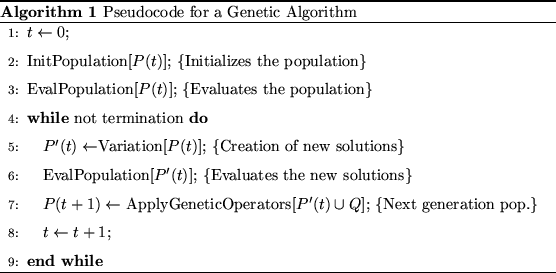
\includegraphics[width=10cm]{fig/ga-pseudocode.png}
\end{figure}

 Para resolver o VRP com GAs, é usual representar cada indivíduo por apenas um cromossomo, o qual é
uma cadeia de inteiros, cada um deles representando um cliente ou um veículo. Então cada
identificador de veículo  representa no cromossomo um separador entre duas rotas, e uma string de
identificadores de strings, representa a sequência das entregas que um veículo deve cobrir dutante
sua rota. Na figura abaixo podemos ver uma representação de uma possível solução pra VRP com 10
clientes e 4 veículos. Cada rota inicia e termina no depósito. Se encontramos na solução dois
identificadores de veículos não separados por algum idenfiticador de cliente, entedenmos que a rota
é vazia, assim, não será necessário usar todos os veículos disponíveis.

\[\underbrace{4-5-2}_{route1}-11-\underbrace{10-3-1}_{route2}-13-\underbrace{7-8-9}_{route3}-12-\underbrace{6}_{route4}\]



 Uma típica função de aptidão  usada para resolver o VRP com GA é $f_{eval}(x) = f_{\max}-f(x),$
onde $f(x)={total}_{distancia}(x)+\lambda sobre_{carga}(x)+ \mu sobre_{tempo}(x)$

 Tanto a função de sobre carga quanto a função de sobre tempo  retornam o quanto de capacidade e
sobre tempo o pode ser permitido. Se nenhuma das restrição da função são violádas, $f$ retorna a
distância total da viágem. Em outros casos tanto capacidade e tempo são pesados com valores
$\lambda$ e $\mu$. A melhor solução mode ter valores fechados para $f_{\max}$, enquanto a solução
que quebra em alguma restrição verá penalizada seu valor de aptidão.

\section{Cozimento Simulado}

 O cozimento simulado (SA) é uma tecnica de relaxamento simulado, o qual tem sua origem na mecânica
estatistica. É baseada numa analogia do processo de cozimento de sólidos, onde um sólido é
esquentado à uma temperatura alta e gradualmente esfriado de modo a cristalizar numa configuração de
baixa energia. SA pode ser visto como um meio de tentar para permitir uma dinâmica básica de
escalada na colina para tambem ser abel a escape ótimo global de soluções de qualidade pobre. SA
guia o pesquisa local original se $\Delta \leq 0$, onde $\Delta = f(x)-f(x_i)$. Permitir a pesquisa
escapar um ótimo local, mover este crescimento os valores da função objetivo são aceitas com uma
probabilidade $e^{-\Delta/T}$ se $\Delta > 0$, onde $T$ é uma paramentro chamado de "temperatura". O
valor de $T$ varia de um valor relativamente grande para um valor pequeno próximo de zero. Esses
valores são controlados por plano frio, o qual especifica o inicio, o valor de temperatura em cada
estante do algoritmo.

 Na iteração $t$ de um cozimento simulado, a solução é desenhada randomicamente em $N(x_i)$. Se
$f(x) \leq f(x_i)$, então $x_{i+1}$ é tomado igual à x; caso contrário

\[x_{i+1}=\begin{cases} 
x & \text{with probability } p_{i}\\ 
x_{i} & \text{with probability }1-p_{i} 
\end{cases},\]

 onde $p_i$ é usualmente uma função decrescente de $t$ e de $f(x)-f(x_i)$. É comum definir $p_i$
como $e^{-\Delta/T}.$

 Há três critérios comuns de parada:

\begin{enumerate}
\item O valor $f^*$ da incombencia $x^*$ não tem decrescimento de no mínimo $\pi_1\%$ para no mínimo
$k_1$ ciclos consecutivos de $T$ iterações;
\item O número de movimentos aceitos tem sido menor que $\pi_2\%$ de $T$ para $k_2$ ciclos
consecutivos de $T$ iterações;
\item $k_3$ de $T$ iterações tem sido executadas.
\end{enumerate}

\section{Pesquisa Tabular}

 O conceito básico de pesquisa tabular (TS) como descrito por {\color{red} referência} é uma
meta-heurística enraigada por outras heurísticas. TS exprora o espaço de solução movento em cada
iteração de uma solução $s$ para a melhro solução num subconjunto das suas vizinhanças $N(s)$.
Contrariando aos métodos clássicos descendentes, a solução atual mode ser determinada de uma
iteração para a próxima. Assim, para ciclos vazios, as soluções possuem alguns atributos de soluções
exploradas recentemente que são declarados temporariamente secretos ou esquecidos. A duração que
estes atributos permanecem secretos é chamado sua tabu-tenure e pode variar sobre diferentes
intervalos de tempo. O estatos de segredo pode overridden se certas condições são encotradas; isso é
chamados o critério de aspiração e acontece, por exemplo, quando a solução secreta é melhor que
alguma solução vista previamente.

 A tendencia de resolução apresentada de uma carta de curso, pode ser lamentavel como uma fonte de
erro mais pode tambem prover uma fonte de ganho. O método de segredo opera neste modo como a esceção
que cursos novos não são escolhidos randomicamente. Em vez de processos de pesquisa secreta acordada
pela suposição que não há pontos em acerto (?) uma nova solução a menos que seja um caminho vazio já
investigado. Isso garante novas regiões de um espaço de solução de problemas será investigada com
uma meta de evitar o mínimo local e ultimamente encontrar a solução desejada.

 A solução inicial é tipicamente criada com alguns heurísticas de inserção baratas. Após criada uma
solução inicial, um trabalho dado é feito para melhora usando pesquisa local com um ou mais
estruturas de vizinhanças e uma estratégia de aceitação melhor. Muitas das vizinhanças usada são
conhecidas e foi previamente introduzidas no contesto de varias construções e heurísticas de
melhorias.

 Aqui, descreveremos três algoritmos diferentes para TS:

\begin{itemize}
\item Segredo granular
\item O processo de memória adaptativa
\item Kelly e Xu
\end{itemize} 

\subsection{Segredo granular}

 A pesquisa secreta granular (GTS) é uma conceito de promessa muito aceita. Foi recentemente
introduzida por {\color{red} referencia} e tem produzido resultados excelentes no VRP. A ideia
essencial por trás do tronco do GTS vem da observação que as arestas longes de uma grafo somente tem
uma probabilidade pequena se pertencem a uma solução ótima. Assim, eliminação de todos os ramos cujo
comprimento excede uma granularidade limiar muitas soluções prometidas nunca serão consideradas pelo
processo de pesquisa. Toch e Vigo sugerem usar $v = \beta \overline{c}$, onde $\beta$ é um parametro
de vergação (?) tipicamente escolhido num intervalo $[1.0, 2.0]$, e $\overline{c}$ é um comprimento
de ramo médio de uma solução obtida por uma heuristica rápida. Se $\beta \in [1.0, 2.0]$, então a
porcentagem de ramos remanescentes no grafo tende a ser $10\%-20\%$ do alcance. Na prática o valor
de $\beta$ é ajustado dinamicamente sempre que o incumbente não tem provado para um conjunto de
iterações, e periódicamente decrescido para seu valor inicial. Visinhança de soluções são obtidas
por faze um número limite de mudanças de ramos dentro da mesma rota ou entre duas rotas. O autor
propõe um processo capacitado de examinar todas as possíveis mudanças num tempo $O(|E(v)|)$, onde
$E=\{(i,j) \in E: c_{ij} \leq v\} \cap I$, e $I$ é um conjunto de ramos importantes tais com suas
incidências para o deposito ou pertencendo a soluções de alta qualidade.

\subsection{O procedimento de memória adaptativa}

 Um dos mais interessantes desenvolvimentos que tem ocorrido na área de TS em anos recentes é o
conceito de Memória Adaptativa desenvolvido por {\color{red} referência}. É largamente usado em TS,
mais sua aplicabilidade não é limitada a este tipo de metaheuristica. Uma memória adaptativa é um
reunião de soluções boas que é dinamicamente atualizado através do processo de pesquisa.
Periodicamente, alguns elementos desta solução são extraidos da reunião e combinados diferentemente
para produzir novas boas soluções. Quando selecionada esta rota, deve ser tomado cuidado ao incluir
o mesmo cliente duas vezes na solução. Essa restrição significa que o processo de seleção
frequentemente termina com uma solução parcial que tera de ser completa usando uma heuristica de
construção. No exemplo ilustrado na figura abaixo, extraindo-se as rotas A, D e H de uma memória de
duas solução resulta numa solução parcial. Rochar e Taillard mostraram que esta aplicação do
processo de memória dinâmica pode melhorar a estratégia de pesquisa. Isso tem os abilitou a obter
duas novas soluções melhores na 14 sentença padrão de comparação de VRP.

\begin{figure}[!ht]
\centering
\includegraphics[width=5cm]{fig/RochatTaillard95.png}
\end{figure}


\subsection{Kelly e Xu}

 Neste caso, {\color{red} referência} considera a troca de vertices entre duas rotas, uma reposição
global dos mesmos veículos de outras rotas, e melhoria local de rotas. A estratégia de reposição
global resolve um modelo de fluxo de rede para otimizar realocação dado o número de vertices em
diferentes rotas. Aproximações são desenvolvidas para calcular o ejeção e inserção de custo,
levando-se a capacidade dos veículos em conta. Otimização de rotas são feitas por meio de 3-opt
mudanças em uma rotina de melhoria TS. O algoritmo é governado por muitos parâmetros os quais são
dinamicamente ajustados através de pesquisa. Uma reunião das melhores soluções é memorizado e
periodicamente usado para reiniciar a pesquisa com novos valores de parâmetros. Sobretudo, esse
algoritmo produz muitas das melhores soluções conhecidas em senteças de referência, mais está longe
de dizer que ele não é tão efetivo quanto outras implementações de TS. Tende a requerer um esforço
computacional carnudo e afinação propriamente seus muitos parametros podem ser problemáticos.



